%
\let\textcircled=\pgftextcircled
\chapter{Confining Structures: Colloidal Gels and Randomly Pinned Spheres}
\label{chap:colloids}

\initial{T}here are many interesting phenomena that arise through the interactions of active particles and their environment. Moreover, the structure of these environments in real-life active systems are often complex  and characterised by random and irregular surfaces. In this chapter, we introduce the two model environmental structures through which we study active particle dynamics: a porous network (modelled by a colloidal gel), and randomly pinned spheres. 
%For the porous network we undertake a multidisciplinary approach, and review the structure in both experiment and simulation in the form of a colloidal gel. It is not possible to recreate randomly pinned sphere in the three-dimensional experimental and therefore this environment is probed computationally.
This chapter is structured as follows: first we introduce the literature pertaining to the creation and modelling of colloidal gels: in section \ref{section:colloids} we introduce colloids formally and outline the advantages of colloidal systems; in section \ref{section:colloidalInteractions} we review the relevant colloidal interactions and how they may be controlled; and in section \ref{section:gels} detail the phase behaviour and structure of colloidal gels. Following this, we conclude in section \ref{section:confinement} with a review of literature regarding the effects of randomly pinned particles within particle suspensions. 

\section{Colloids}
\label{section:colloids}

Insoluble particles suspended in a fluid phase are known as colloids. Colloidal particles are predominantly defined by their size \cite{lu2013}. This lengthscale is essential to the dynamics of colloids as it allows them to be suspended in the fluid phase through the thermal fluctuations of Brownian motion. Colloids  considered along with the fluid phase are known as colloidal suspensions. Colloidal suspensions are a common form of matter, found in both natural materials such as milk and blood, as well as artificial materials such as paints and inks.

\textit{Colloids as model systems ---} colloids have a long history as experimental model systems. Thanks to their size and diffusive time scales, they provide an accessible model system for many applications, as they can be observed in real time with microscopy techniques.
Colloids are often used to approximate atomic or molecular systems, and can be made to exhibit similar phase behaviours such as solids, liquids and gases. In fact the "colloidal atom" has been given rigorous justification \cite{mcmillan1945}.
Moreover, through modification of their surface chemistry and manipulation of their surrounding environment, colloids can be designed to possess bespoke and tuneable interactions. This allows for colloids to provide the basis for the study of a wide-range of systems and phenomena including: gels \cite{zaccarelli2007}, glasses \cite{poon2004}, crystals \cite{yethiraj2003}, and self-propelling particles \cite{bechinger2016a}. 
Finally, given that the particle interactions are well understood and can be described by classical interactions; these systems are highly amenable to simulation and thus many works take a multidisciplinary approach where simulations are matched to experiments.


\section{Colloidal interactions}
\label{section:colloidalInteractions}

Colloids dispersed in a medium and undergoing Brownian motion will collide. As a result of certain properties (electrical or otherwise) belonging to the colloids or their surrounding medium, a suspension of colloids can aggregate irreversibly or remain in a stable dispersion \cite{lekkerkerker2011}. As mentioned previously, one significant advantage to working with colloidal systems is the ability to control the particle interactions and bias these systems to certain behaviours. In this section we review the interactions relevant to this work, namely: the van der Waals, electrostatic, hard sphere, and depletion interactions.


\subsection{Van der Waals interaction}

Van der Waals forces are present in all atoms and molecules. These forces originate as a result of the cooperative oscillation of electron clouds of atoms at small separations \cite{lekkerkerker2011}. For two colloids suspended in a solvent at close range, the interactions in between all of the atoms that constitute their volume sum to create an effective interaction known as the colloidal van der Waals interaction. The strength of this interaction is dependant on both the dielectric properties of the colloids and the surrounding solvent. For two spherical colloids of diameter $\sigma$ at a separation $r$, the colloidal van der Waals interaction takes the following form:

\begin{equation}
U_{\textrm{VdW}}(r)=-\frac{A_{H}}{12}\left[\frac{\sigma^{2}}{r^{2}-\sigma^{2}}+\frac{\sigma^{2}}{r^{2}}+2 \ln \left(\frac{r^{2}-\sigma^{2}}{r^{2}}\right)\right]
	\label{eq:VdW}
\end{equation}

\noindent where $A_H$ is the Hamaker constant \cite{lekkerkerker2011}. The Hamaker constant collects material properties of the colloids and their surrounding medium. This value can be determined with Lifshitz's approximation in which $A_H$ is dependant on the differences in the refractive index and the dielectric constant between the colloids and the medium \cite{prieve1988}.

 The van der Waals interaction is very strong at small separations and unless counteracted by some other forces, it will induce particle aggregation at sufficient densities. However, this force can be significantly reduced if the difference in the refractive index or the dielectric constant of the colloids and the surrounding medium is close to zero, as this causes $A_H$ in eq. \ref{eq:VdW} to approach zero. 
 
 


\subsection{DLVO interaction}
A charged colloid suspended in solution will incur a response in the surrounding ion distribution. Counter-ions (baring the opposite charge) are attracted to the particle surface, while co-ions (same charge as the colloid) are repulsed, and at long-range the ion distribution holds an average constant value \cite{lekkerkerker2011}. A schematic of this inhomogeneous layer is shown in Fig. \ref{fig:DLVO}a. This layer is known as a double layer, its thickness is dependant on the bulk solvent ion concentration and therefore an increase in the number of ions increases the screening of the colloidal charge \cite{lekkerkerker2011}. 

If the particle separation of two colloids becomes small enough that their respective double layers overlap, the resultant pair-potential produces a repulsive pressure. This repulsive pair potential can be expressed through a modification of the Coulombic potential known as the Yukawa potential:

\begin{equation}
	U_{\textrm{Yuk}}(r) \propto \frac{\exp (-r / \lambda_D)}{r}
	\label{eq:Yuk}
\end{equation}

\noindent where $\lambda_D$ is the Debye screening length which corresponds to the length scale over which the double layer repulsive force acts. 

\begin{figure*}
	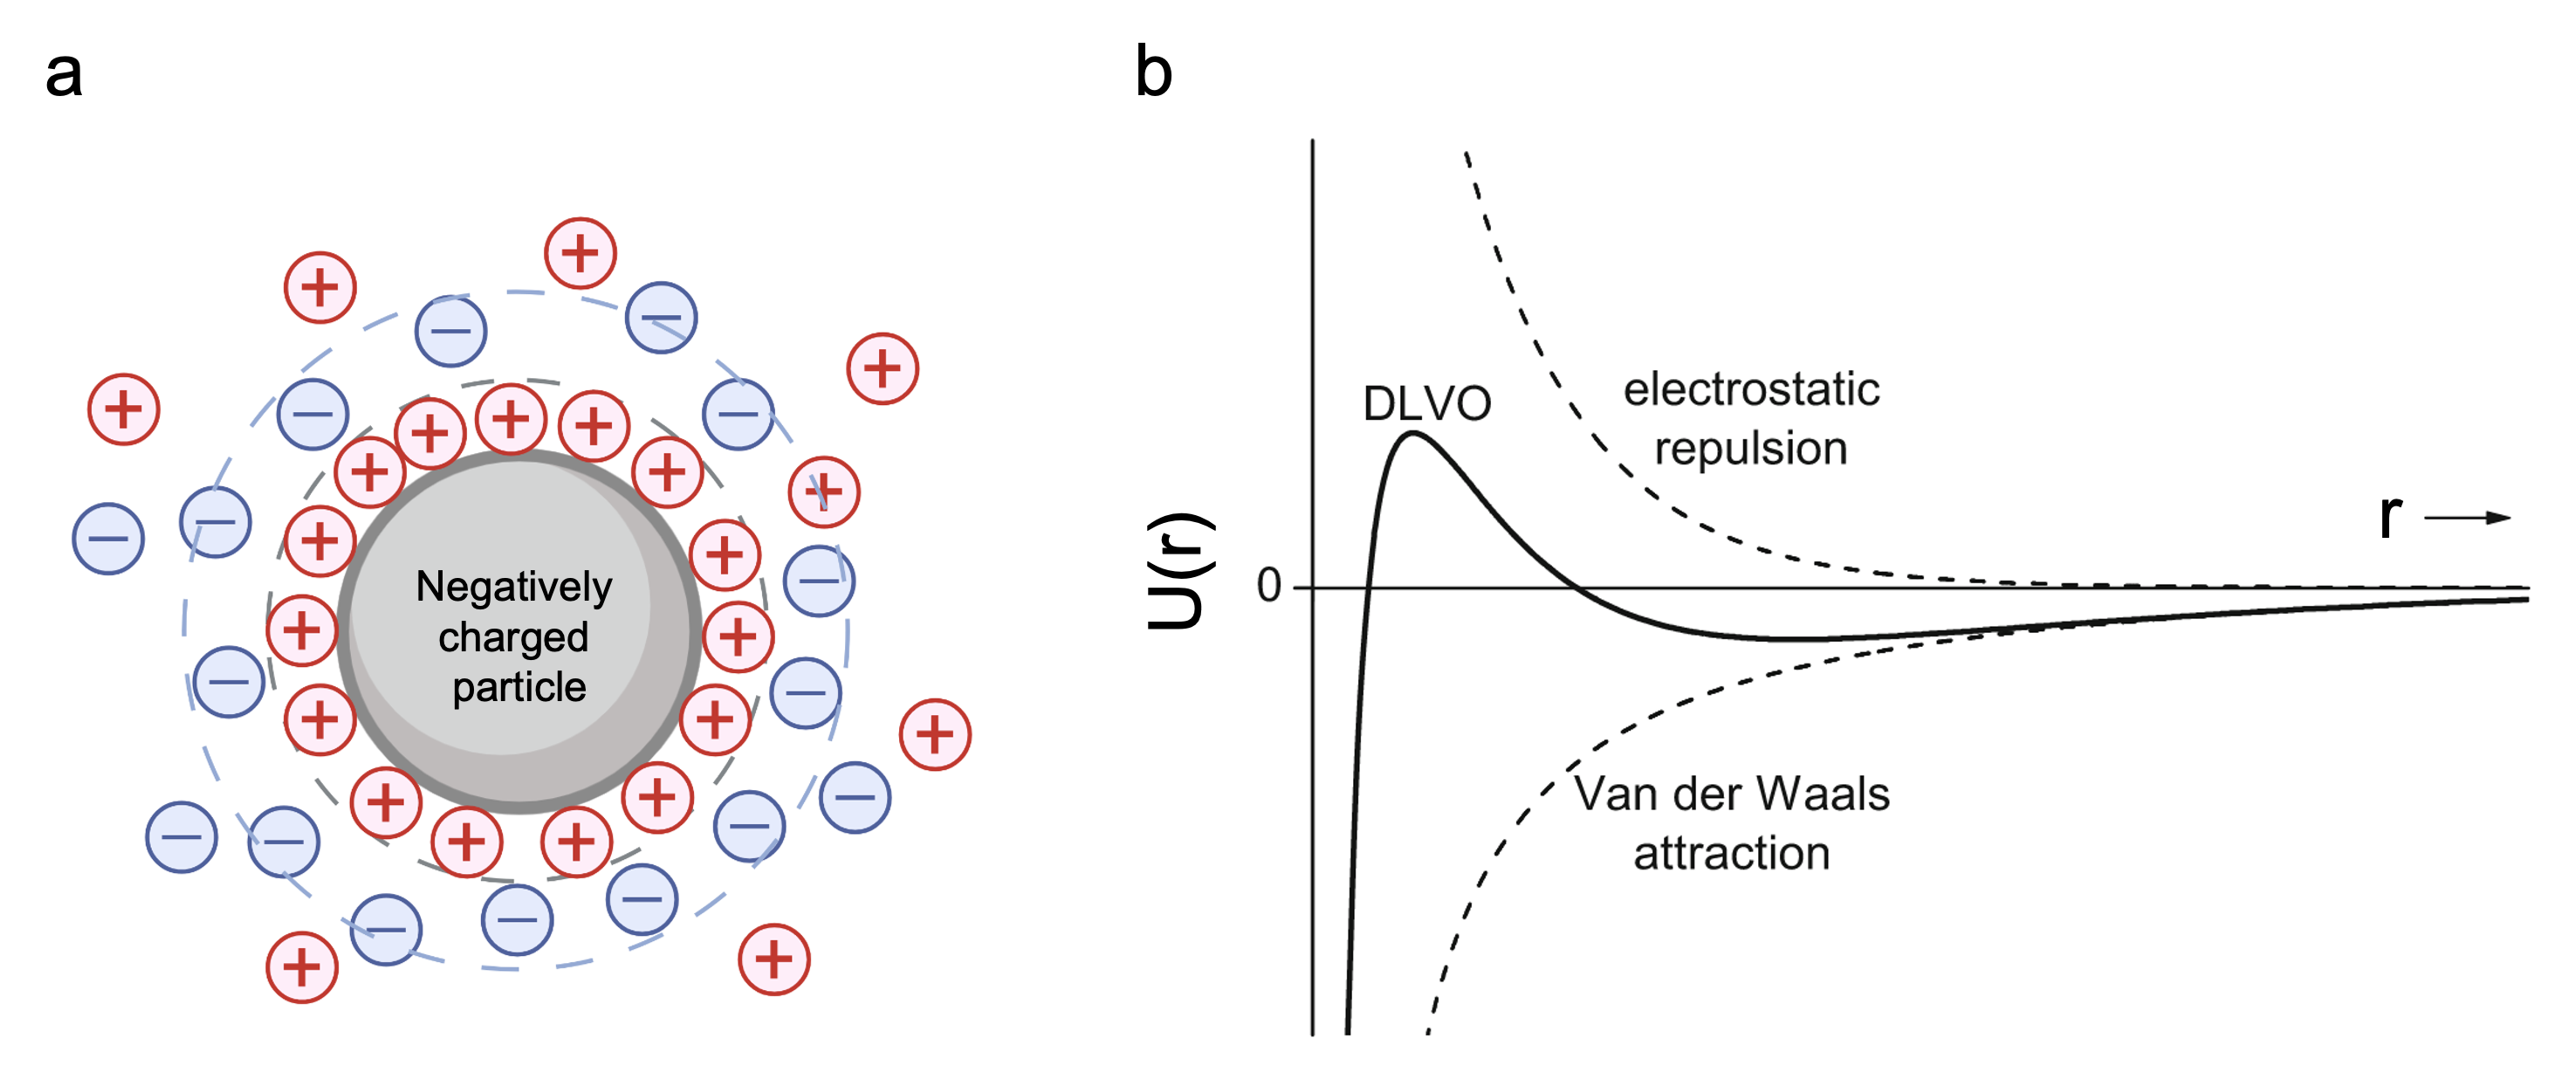
\includegraphics[width=\linewidth]{chapters/colloids/figsColloids/figDLVO.png}
	\caption[Electric double layer and the DLVO potential.]{Electric double layer and the DLVO potential. \textbf{a} A negatively charged colloid (grey) attracts counter-ions (red) and co-ions (blue). \textbf{b} The DLVO potential is the sum of Van der Waals attractions and double layer electrostatic repulsion. DLVO plot adapted from ref. \cite{lekkerkerker2011}.}
	\label{fig:DLVO}
\end{figure*}

A pair of charged colloids will experience the effects of both van der Waals and double layer interactions and therefore these two interactions are often compounded into a superposition of the two known as the DLVO interaction. Assuming these potentials can be summed, the DLVO interaction takes the following form:

\begin{equation}
	U_{\textrm{DLVO}} = U_{\textrm{VdW}} + U_{\textrm{Yuk}}
\end{equation}

\noindent A typical resultant DLVO potential is illustrated in Fig. \ref{fig:DLVO}b along with its constituent potentials. This potential can be manipulated through control of the salt (and therefore the ion) concentration of the solvent: Low salt concentrations favour the double layer and lead to a stable colloidal suspension; whereas very high salt concentrations favour the van der Waals interaction and can cause irreversible aggregation \cite{lekkerkerker2011}.

\subsection{Hard sphere interactions}
\label{section:HardSpheres}
For a pair of interacting spherical colloids, the simplest description is the hard sphere interaction. In this scenario, the colloids possess no charge interactions, nor any other attractive or repulsive influences, the only rule imposed on to the particles is that they cannot overlap. For mono-disperse spheres of diameter $\sigma$, the hard sphere pair-potential is the following:


\begin{equation}
 U_\mathrm{HS}(r) = \begin{cases}
\infty & r < \sigma \\%&\text{se $\omega\in A$}\\
0 & r \geq \sigma   
\end{cases}
\label{eq:HSinteraction}
\end{equation}

\noindent where $r$ is the particle separation. 

Colloidal particles are subject to Brownian motion, and therefore dilute suspensions of hard spheres exhibit a diffusive disordered gas-like state. As a function of increasing particle density; hard sphere colloids undergo a series of transitions from the disordered gas-like state, to a dense fluid-like state, and eventually to a crystalline solid through an entropy driven mechanism \cite{wood1957,alder1957}.

\begin{figure*}
	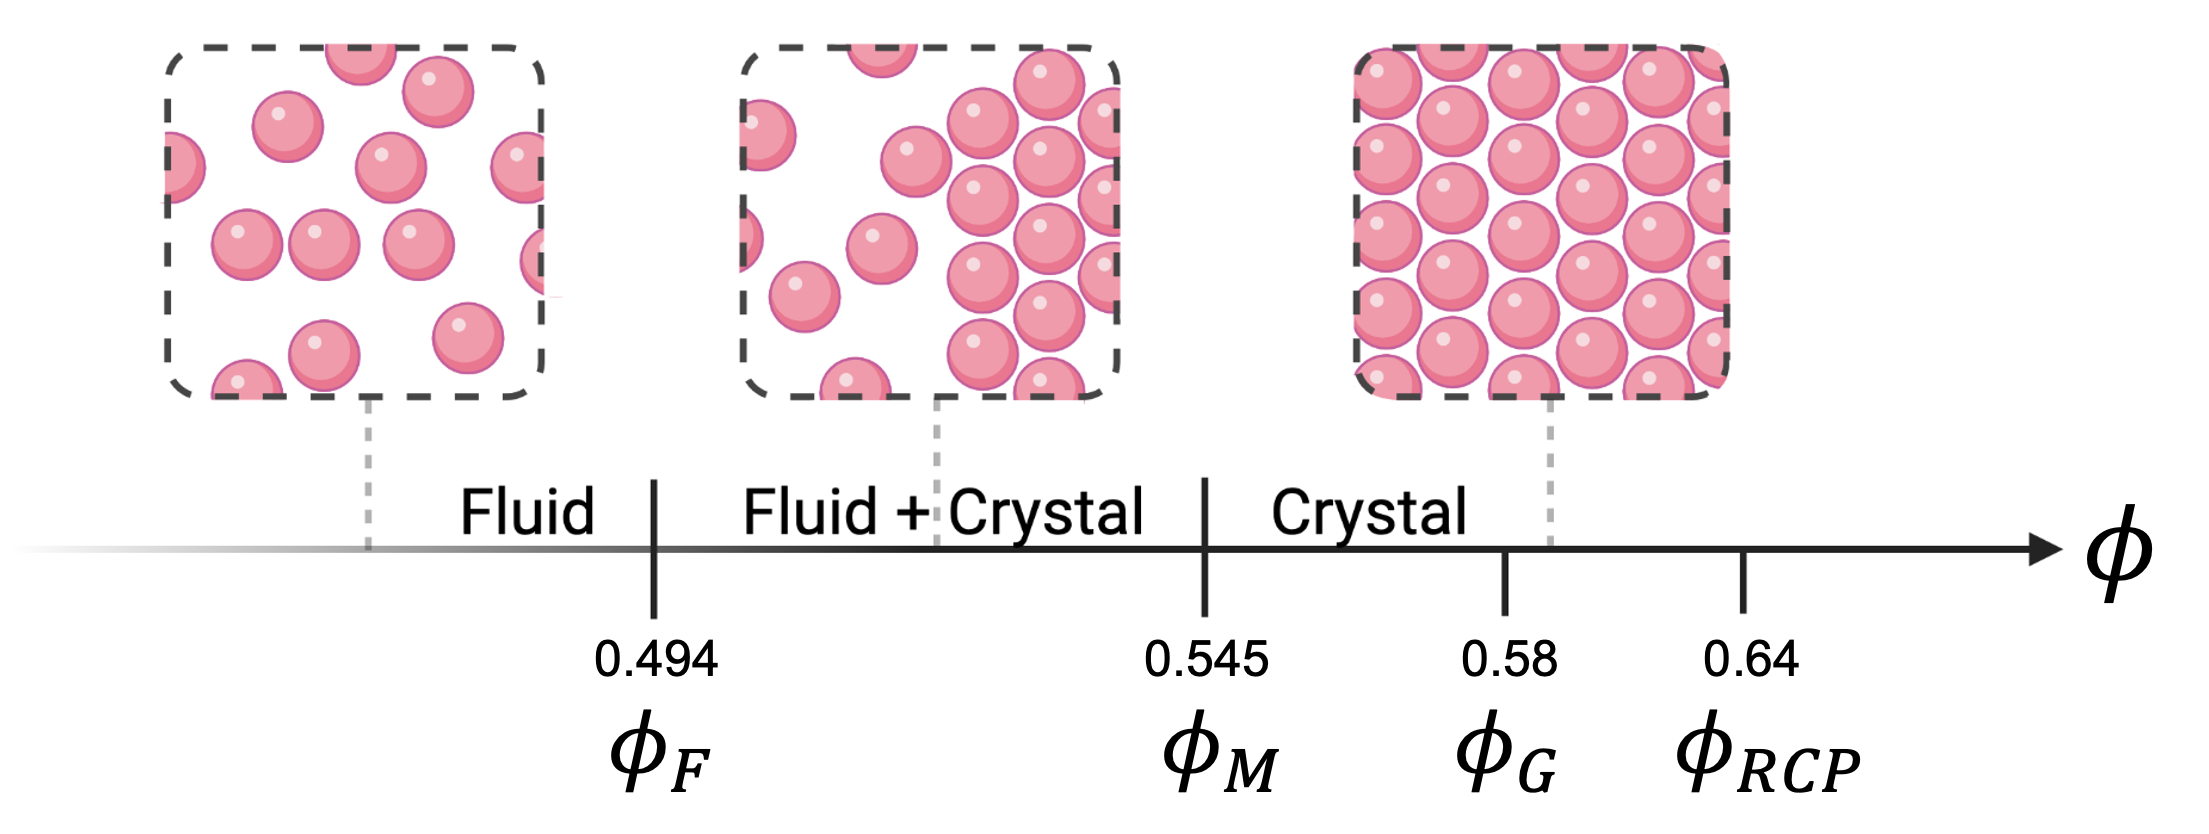
\includegraphics[width=\linewidth]{chapters/colloids/figsColloids/figHardSpheres.png}
	\caption[The hard sphere phase diagram.]{The hard sphere phase diagram. As a function of the volume fraction $\phi$, hard spheres (pink) exhibit different phases. Important volume fractions: freezing $\phi_F$, melting $\phi_M$, the glass transition $\phi_G$, and random close-packing $\phi_{\textrm{RCP}}$.}
	\label{fig:HardSpheres}
\end{figure*}


Given that the nature of this interaction arises from the excluded volumes of the colloids, the main parameter governing an ensemble of hard spheres is the volume fraction $\phi$. This parameter is the fraction of the system volume taken up by the colloids and can be expressed with the following relation:

\begin{equation}
	\phi = \frac{\pi \sigma^3}{6}\frac{N}{V},
	\label{eq:volumeFraction}
\end{equation}

\noindent where $N$ is the total number of particles and $V$ is the system volume. The simplicity of this system makes it highly amenable to theoretical description and analysis via simulation \cite{boublik1970,rintoul1996}. This has resulted in a large number of studies focussed on this system in past decades and as a result the phase diagram of hard spheres as a function of volume fraction is well known \cite{hoover1968} (Fig. \ref{fig:HardSpheres}). 
This one-dimensional phase diagram shows the progression of hard spheres undergoing a first order phase transition to a crystalline state. Marked on this figure are the typical volume fractions for freezing ($\phi_F = 0.494$) and melting ($\phi_M = 0.545$) \cite{hoover1968}, between which the system exhibits liquid-crystal coexistence. Other notable points are random close packing ($\phi_{\textrm{RCP}} = 0.64$), which corresponds to the maximum volume fraction of randomly packed particles. Furthermore, should a hard sphere system exceed $\phi_G =  0.58$ without crystallising, it will slowly transition to a glass; a disordered non-ergodic solid state \cite{palberg2016}.



Regarding crystallisation in this system, mono-disperse hard spheres will crystallise into two polymorphs: the face-centred cubic lattice (FCC), and hexagonal close packing (HCP). These structures are depicted in Fig. \ref{fig:HardSpheres}. 


\begin{figure*}
	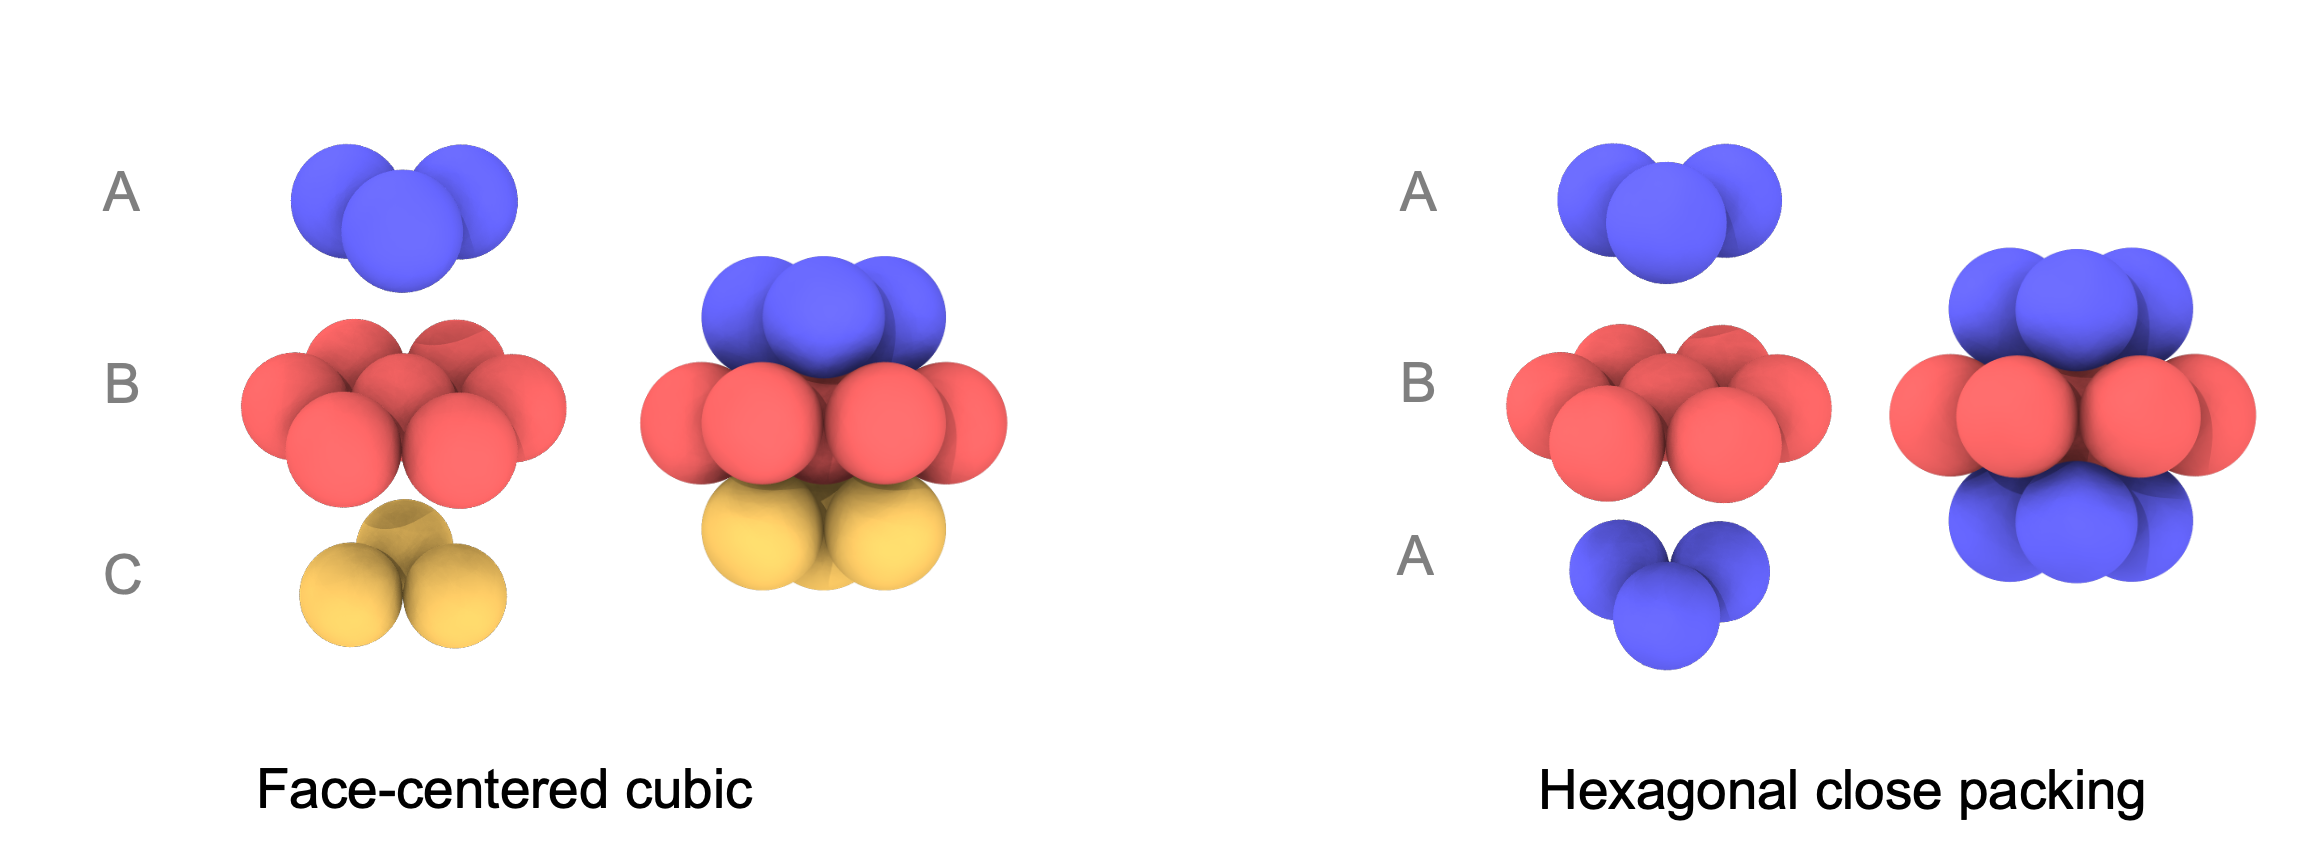
\includegraphics[width=\linewidth]{chapters/colloids/figsColloids/figFCCvsHCP.png}
	\caption[Polymorphs of hard sphere crystals]{Polymorphs of hard sphere crystals. The two polymorphs differ in their stacking of hexagonal layers: the face-centered cubic (FCC) crystal has an ABC structure, while hexagonal close packing (HCP) crystals have an ABA structure.}
	\label{fig:FCCvsHCP}
\end{figure*}

The difference between these two polymorphs in all relevant thermodynamic quantities (such as free-energy, nucleation barrier, and stacking free-energy) is negligibly small (within $10^{-3}$ $k_B T$ per particle for all cases) \cite{woodcock1997,pronk1999}. 
When hard spheres nucleate into crystalline structures in equilibrium systems, the resultant polymorph make-up of the crystal will be a near equal mix of the two structures. This is a result of two factors: first is that based on the Ostwald step rules of phases \cite{ostwald1897}, we know that the first solid that nucleates in a system is not necessarily the most thermodynamically stable, but the state of nearest free energy to the initial state. Second is that as a result of the difference in stacking entropy between the FCC and HCP structures, there is a slight favouring of FCC nuclei \cite{pronk1999,leoni2021,coli2021}.
  


\subsection{Depletion interaction}

\begin{figure*}
	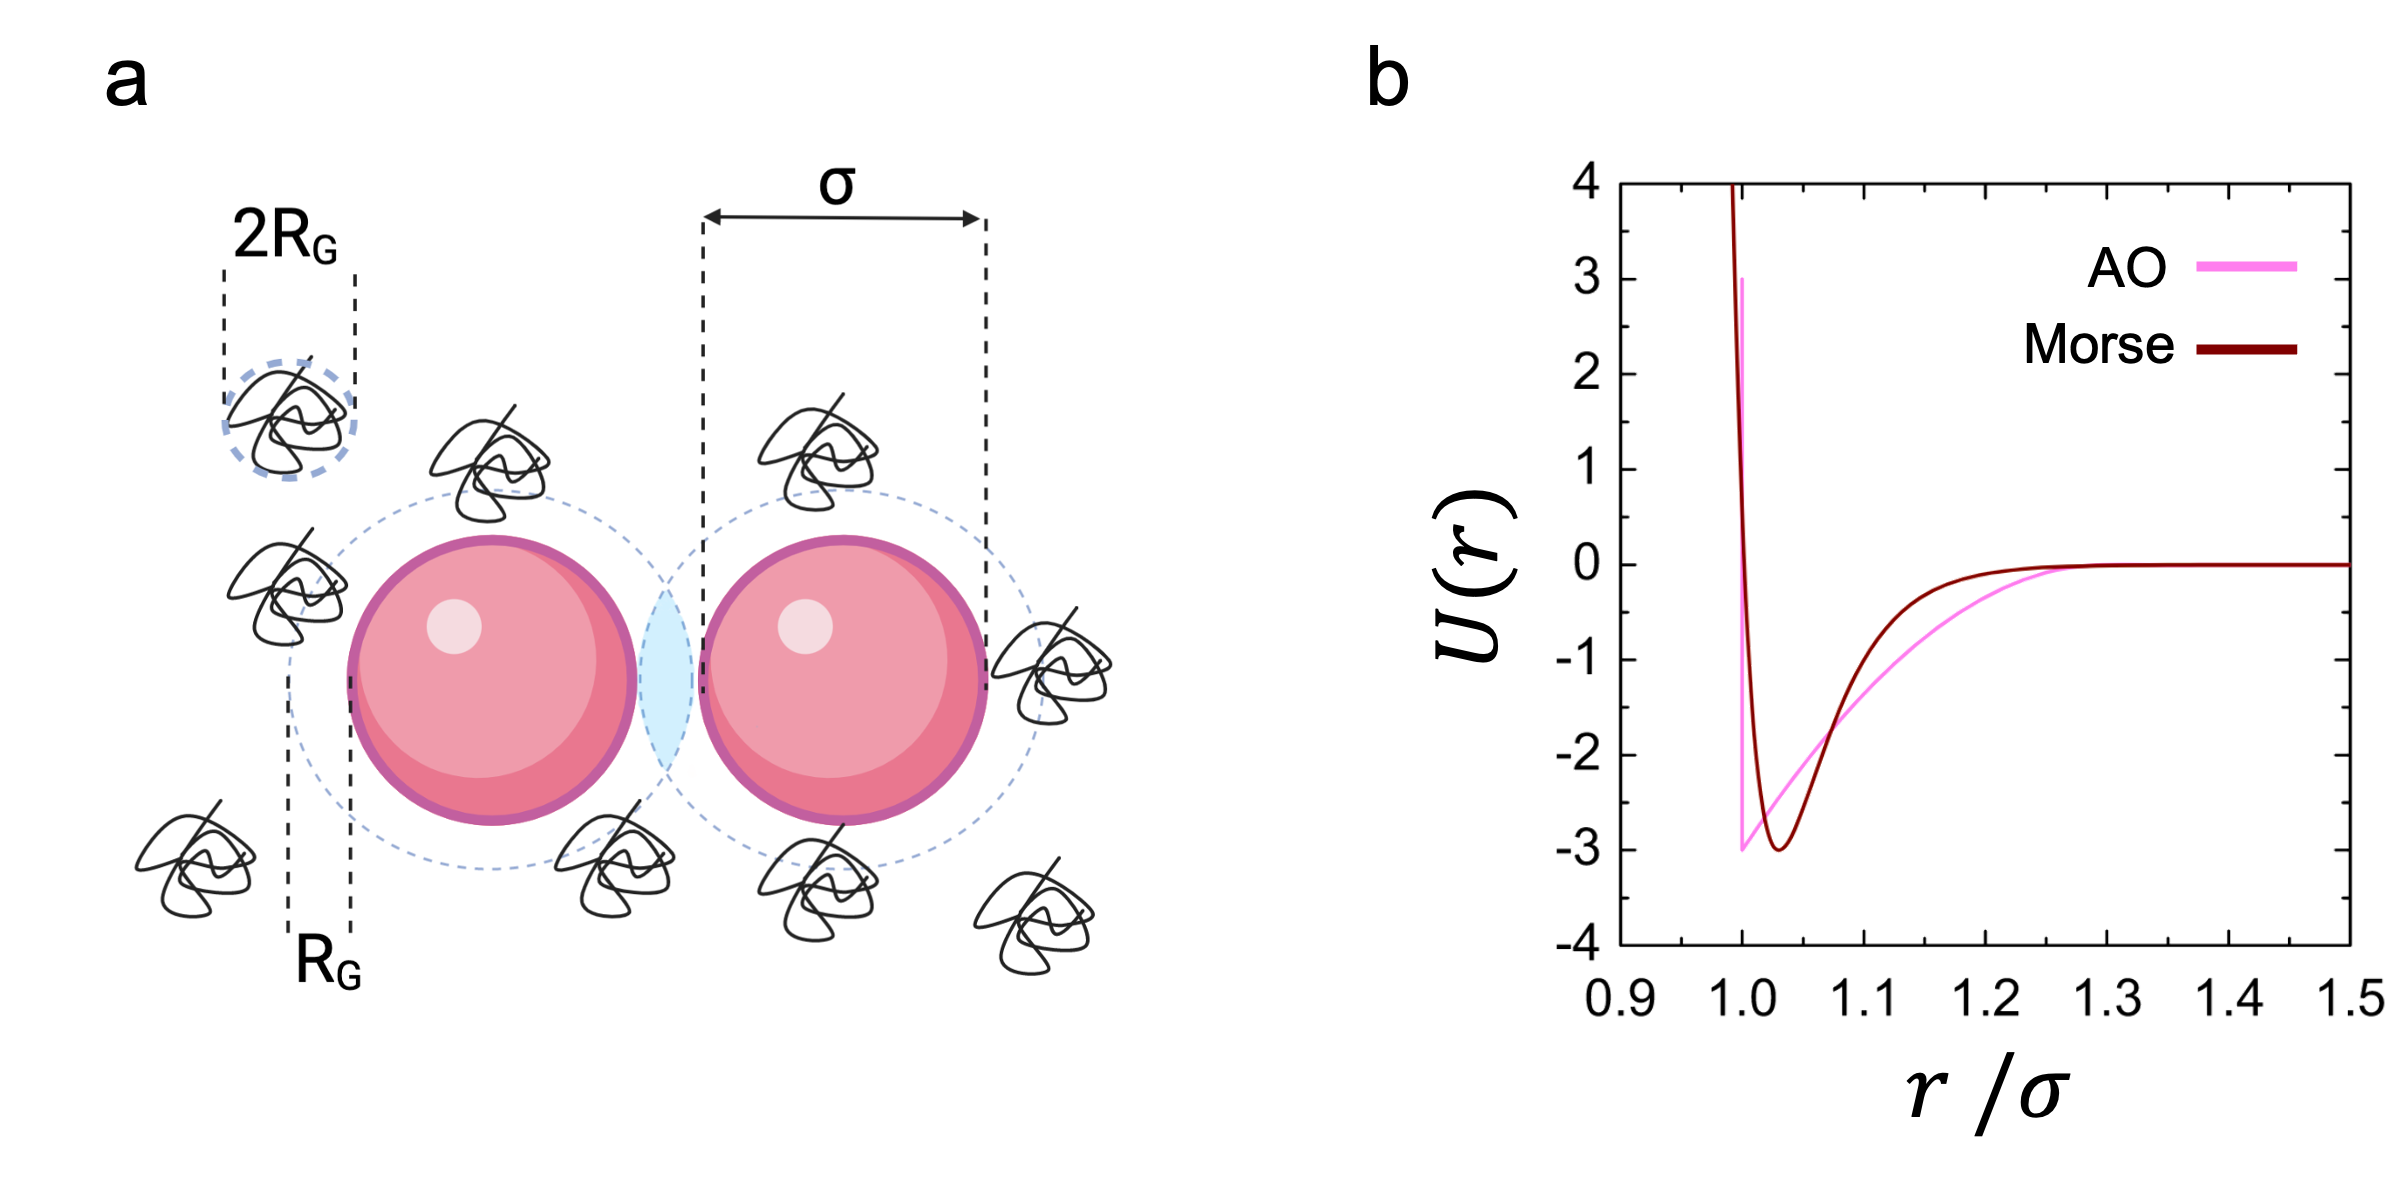
\includegraphics[width=\linewidth]{chapters/colloids/figsColloids/figDepAO.png}
	\caption[The depletion interaction]{The depletion interaction. \textbf{a} A schematic showing the mechanism for the osmotic pressure responsible for depletion attraction. The colloids (pink) are each surrounded by an exclusion zone of thickness $R_G$ from the particle surface. Particles with a separation of less than $\sigma + 2R_G$ produce an excluded volume (blue) that is inaccessible to the polymer depletants. \textbf{b} The two primary depletion pair-potentials: the Asakura-Oosawa interaction (pink) and the Morse interaction (brown), adapted from ref. \cite{taffs2010a}.}
	\label{fig:DepAO}
\end{figure*}

The addition of a non-adsorbing polymer to a colloidal suspension induces an effective attractive interaction by way of \textit{depletion}. Here the term depletion refers to the preferential exclusion of the polymer (the depletant) from proximity with the colloids. The effective attraction between colloids derives from an anisotropic osmotic pressure that arises from entropy gain in the polymer solution. The mechanism through which this attraction arises in demonstrated in Fig. \ref{fig:DepAO}a.


Here the colloids are hard particles as described in section \ref{section:HardSpheres} suspended in a solution containing polymer. Assuming the polymer is dissolved in a "good" solvent \cite{berry1966,royall2007a}, the random walk of polymer chains will result in an approximately spherical configuration with a radius known as the radius of gyration $R_G$. In Fig. \ref{fig:DepAO}a, drawn around the colloids is a dotted line marking a distance equal to $R_G$ from the particle surface. This is termed the exclusion zone and defines the boundary beyond which the centre of the spherical polymer cannot pass due to the hard sphere nature of the colloid. Should any two colloids travel within close proximity of each other such that their exclusion zones overlap, this resulting overlap volume is then completely inaccessible to any polymer in the system. This creates a situation in which the density of polymer between the colloids is lower than that of the bulk. This imbalance creates a density gradient that drives an anisotropic osmotic pressure acting to bring the colloids together. 

The depletion force is often described as an entropic force. The overlap of exclusion zones as colloids come together increases the free volume available to the polymers corresponding to an increase in their configurational entropy \cite{lekkerkerker2011}.
This effective interaction can be modelled as a pair-wise interaction (assuming ideal polymers), and is known as the Asakura-Oosawa (AO) model:

\begin{equation}
	\beta U_{\mathrm{AO}}(r)=\left\{\begin{array}{ll}\infty & \text { for } r>\sigma \\ -\frac{\pi \sigma_{P}^{3} z_{\mathrm{p}}}{6} \frac{(1+q)^{3}}{q^{3}}\left[1-\frac{3 r}{2(1+q) \sigma}+\frac{r^{3}}{2(1+q)^{3} \sigma^{3}}\right] & \text { for } \sigma \leq r < \sigma+2R_G \\ 0 & \text { for } r \geq \sigma+2R_G\end{array}\right.
	\label{eq:AO}
\end{equation}

\noindent where $q$ is the size ratio between the polymer and the colloids $q = 2R_G / \sigma$, and $z_p$ is the polymer \textit{fugacity}.  The fugacity represents the number density of ideal polymer in a reservoir of equal chemical potential to the primary system \cite{royall2021}. The model described in  eq. \ref{eq:AO} defines an attraction that is subject to two main parameters: the size ratio, and the concentration of polymer. Both of these parameters affect the phase behaviour of systems of colloid and polymer mixtures, this phase behaviour is detailed later in section \ref{section:colloidPolymerMixture}.

For computational studies of systems with depletion interactions the AO interaction is often approximated with a continuous potential, such as the Morse interaction:

\begin{equation}                                                                                                                                                                                                                                                                                                                                                                                                                                                                                                                                                                                                                                                                                                                                                                                                                                                                                                                                                                                                                                                                                                                                                                                                                                                                                                                                                                                                                                                                                                                                                                                                                                                                                                                                                                                                                                                                                                                                                                                                                                                                                                                                                                                                                                                                                                                                                                                                                                                                                                                                                                                                                                                                                                                                                                                                                                                                                                                                                                                                                                                                                                                                                                                                                                                                                                                                                                                                                                                                                                                                                                                                                                                                                                                                                                                                                                                                                                                                                                                                                                                                                                                                                                                                                                                                                                                                                                                                                                                                                                                                                                                                                                                                                                                                                                                                                                                                                                                                                                                                                                                                                                                                                                                                                                                                                                                                                                                                                                                                                                                                                                                                                                                                                                                                                                                                                                                                                                                                                                                                                                                                                                                                                                                                                                                                                                                                                                                                                                                                                                                                                                                                                                                                                                                                                                                                                                                                                                                                                                                                                                                                                                                                                                                                                                                                                                                                                                                                                                                                                                                                                                                                                                                                                                                                                                                                                                                                                                                                                                                                                                                                                                                                                                                                                                                                                                                                                                                                                                                                                                                                                                                                                                                                                                                                                                                                                                                                                                                                                                                                                                                                                                                                                                                                                                                                                                                                                                                                                                                                                                                                                                                                                                                                                                                                                                                                                                                                                                                                                                                                                                                                                                                                                                                                                                                                                                                                                                                                                                                                                                                                                                                                                                                                                                                                                                                                                                                                                                                                                                                                                                                                                                                                                                                                                                                                                                                                                                                                                                                                                                                                                                                                                                                                                                                                                                                                                                                                                                                                                                                                                                                                                                                                                                                                                                                                                                                                                                                                                                                                                                                                                                                                                                                                                                                                                                                                                                                                                                                                                                                                                                                                                                                                                                                                                                                                                                                                                                                                                                                                                                                                                                                                                                                                                                                                                                                                                                                                                                                                                                                                                                                                                                                                                                                                                                                                                                                                                                                                                                                                                                                                                                                                                                                                                                                                                                                                                                                                                                                                                                                                                                                                                                                                                                                                                                                                                                                                                                                                                                                                                             U_{\textrm{Morse}}\left(r\right)= \varepsilon_{\textrm{Morse}} \exp \left[a_{0}\left(\sigma-r\right)\right]\left(\exp \left[a_{0}\left(\sigma-r\right)\right]-2\right)
    \label{eq:Morse}
\end{equation}

\noindent where $a_0$ is a range parameter, and $\varepsilon_{\textrm{Morse}}$ is the depth of the potential well. This attractive pair-potential has a variable range ($a_0$) that can be tuned to match the AO interaction for a given size ratio or polymer concentration (Fig. \ref{fig:DepAO}b). Moreover, it has been shown that under certain conditions the Morse potential has out-performed the AO interaction when it comes to reproducing the higher-order structure of colloid-polymer mixtures \cite{taffs2010, royall2021}.


\section{Colloidal gels}
\label{section:gels}

A gel is a material that lies between liquid and solid states, and displays properties of both. They are comprised of low-density cross-linked structures that permeate through a liquid phase. These three-dimensional cross-linked structures promote solid-like behaviour such that the systems do not flow in the steady-state. However, their liquid phase remains diffusive and will allow for the permeation of small molecules or particles \cite{tokita2016}. In terms of structure, the branching networks are typically random and fractal in nature, with an associated lengthscale \cite{zaccarelli2007}. 

It is for this structure that colloidal gels were chosen as one of the model confining environments in this work. The solvent phase surrounding the colloidal network is a series of random percolating channels of varying breadth and connectivity. In this way, the space shares characteristics with porous soils and internal cell structures, the natural environments of mesoscale active matter. Furthermore, as we have seen in the previous section, colloidal systems can be well controlled through various interactions and thus provide an amenable system for experimentation.

Colloidal gels are often formed though depletion interactions, where the addition of a polymer species incurs a self-assembly process in which the colloids become aggregated into disordered branching networks. A colloidal gel is one phase of a system known as the colloid-polymer mixture. In the following section we expound the phase behaviour of this system and detail the process through which colloidal gels are formed.


\begin{figure*}
	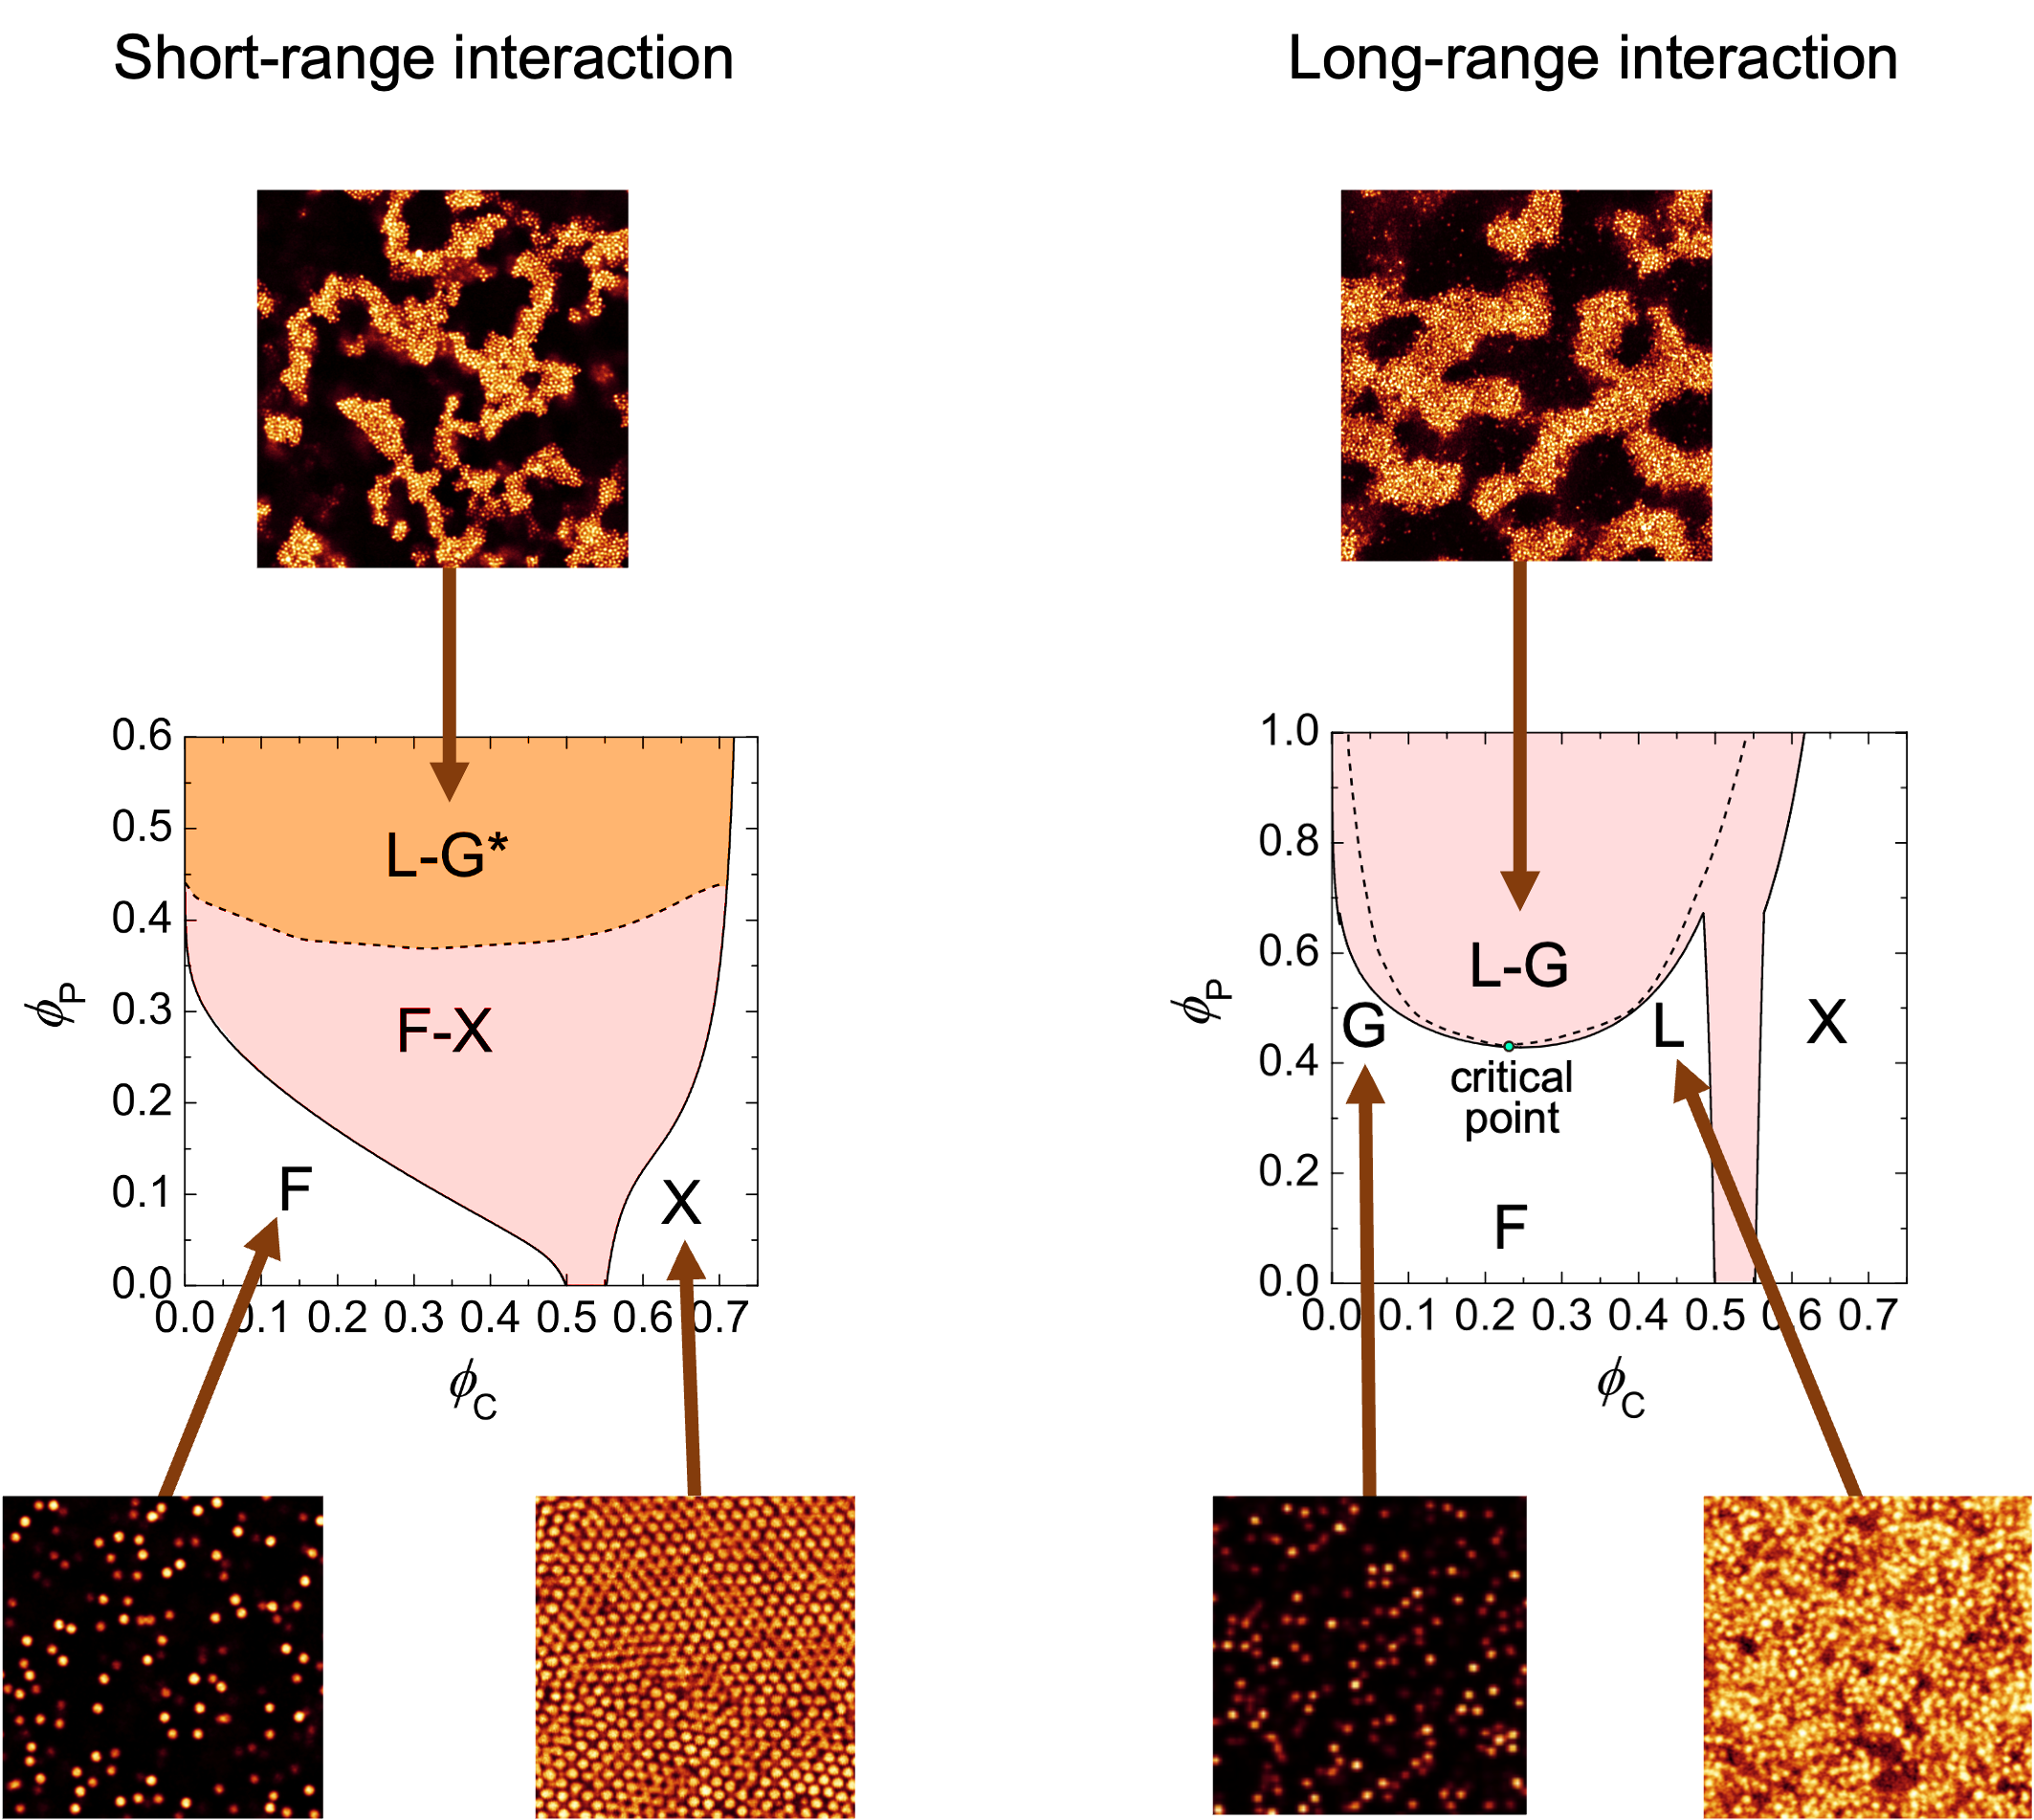
\includegraphics[width=\linewidth]{chapters/colloids/figsColloids/figGel_PD.png}
	\caption[Phase diagrams of the colloid-polymer mixture]{Phase diagrams of the colloid-polymer mixture. Left: short-range interaction $q = 0.18$. Right: long-range interaction $q=0.45$. Symbols correspond to phases: G = gas, F = fluid, L = liquid, X = crystal. The colloidal gel corresponds to the phase of liquid-gas coexistence, where L-G* is a metastable phase. Solid lines mark bimodal lines, dotted lines enclose regions of spinodal decomposition. Adapted from ref. \cite{ivlev2012}.}
	\label{fig:Gel_PD}
\end{figure*}



\subsection{The colloid-polymer mixture}
\label{section:colloidPolymerMixture}

Colloidal particles in the presence of non-adsorbing polymer results in a colloid-polymer mixture. This system exhibits a variety of phases dependant on the both the colloid volume fraction $\phi_c$ and the polymer volume fraction $\phi_p$. Where $\phi_c$ is given by the hard-sphere volume fraction defined in eq. \ref{eq:volumeFraction}, and $\phi_p$ is given by $\phi_p = 4\pi R_{G}^{3} \rho_p / 3$, where $\rho_p$ is the polymer number density. 

In addition to the respective volume fractions, the phase behaviour of the colloid-polymer mixture is dependant on the size-ratio $q$, which determines the range of the interaction: $q<0.3$ corresponds to short-range interactions and $q>0.3$ results in long-range interactions \cite{gast1983}. Phase diagrams for two values of $q$ are shown in Fig. \ref{fig:Gel_PD} providing examples of short-range ($q = 0.18$) and long-range ($q = 0.45$) interactions.

\textit{Short-range interactions ---} for $q<0.3$ and low $\phi_p$, the system exhibits three phases as a function of increasing $\phi_c$: transitioning from a colloidal fluid; to a phase of fluid-crystal coexistence; and finally to a colloidal crystal. At high $\phi_p$ the polymer-induced depletion interaction brings about a metastable phase of liquid-gas coexistence.  In this phase the system demixes into a percolating network of colloid rich branches surrounded by a viscous polymer-rich solvent --- a colloidal gel.

\textit{Long-range interactions ---} for $q>0.3$ the region of liquid-crystal coexistence is significantly narrowed in comparison with the short-range interaction. Furthermore, mixtures with long-range interactions contain critical and triple points \cite{lekkerkerker1992}, with the phase behaviour of this system in general demonstrating characteristics analogous to simple atomic materials \cite{gast1983,vincent1988}. 

\textit{Gelation via arrested phase separation ---} the gelation of a colloid-polymer mixture typically occurs through \textit{spinodal decomposition}, meaning that the system undergoes a spontaneous and immediate phase change without nucleation. 
Once the demixing process begins, these phases undergo dynamical arrest where as a result of the effective attraction; the system becomes quenched. This dynamical arrest leads to the formation of the gel and is an example of viscoelastic phase separation \cite{tanaka2000}, which describes systems for which the demixed phases possess markedly differing viscosities.
Following phase separation, the system is constrained to a much reduced set of local potential-energy minima, and forms in a solid-like material \cite{royall2008,royall2021}. Gels that form via this process are considered to be far from equilibrium, as this arrested structure persists rather than separating into colloid-rich and colloid-poor states, as would be the case in thermal equilibrium \cite{poon2002}.
In Fig. \ref{fig:Gel_PD} the region within which the system undergoes gelation is marked as liquid-gas coexistence (L-G). However, L-G is an equilibrium state corresponding to full demixing, which does not occur for spinodal gels on experimental timescales. 


\section{Random media}
\label{section:confinement}


Now we move on from colloidal gels to the second confining structure relevant to this thesis: randomly pinned spherical particles. The structure of this system is distinct from the branched network of colloidal gels, where instead of elongated channels; the spheres are pinned randomly resulting in a unique geometry and a differing lengthscale.

\begin{figure*}
	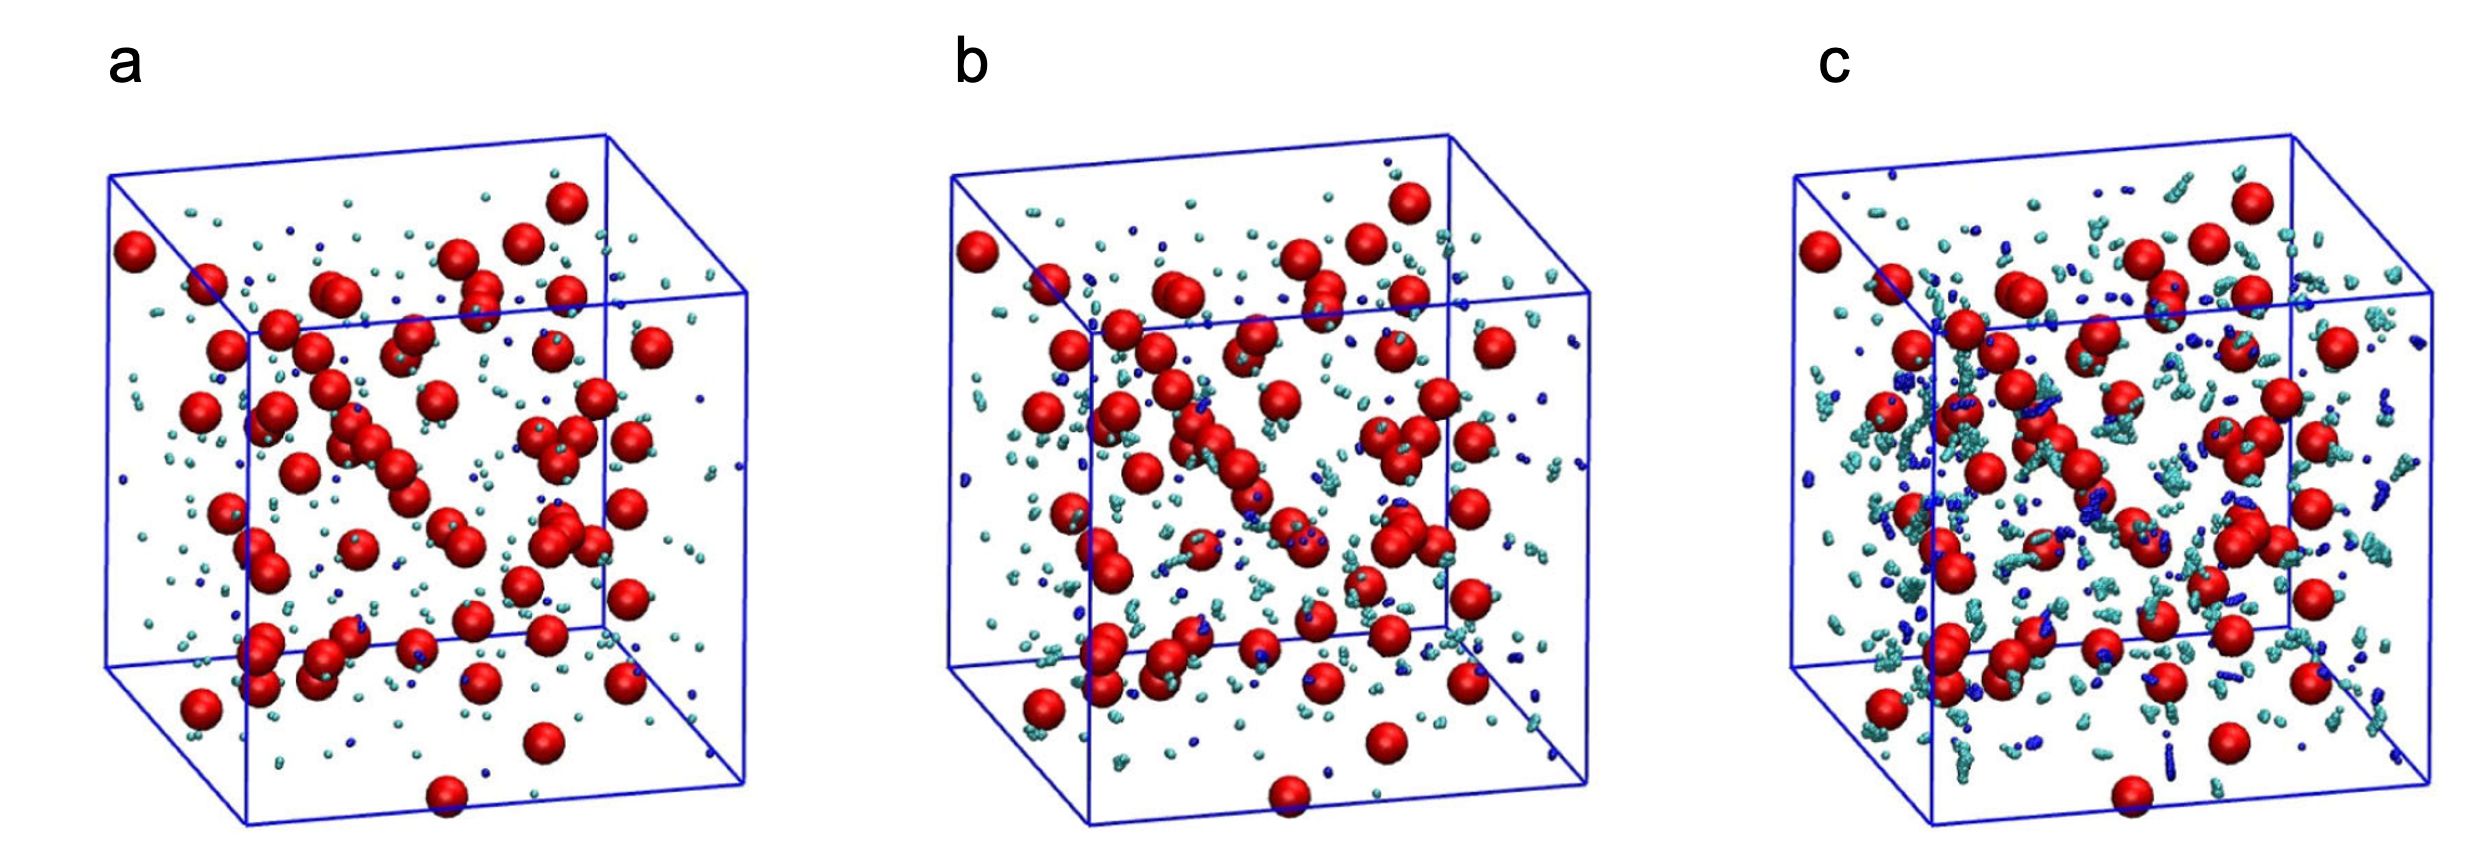
\includegraphics[width=\linewidth]{chapters/colloids/figsColloids/figPinning_TJ.png}
	\caption[Localisation in a random pinning fluid.]{Localisation in a random pinning fluid. Free particles in a binary Lennard-Jones fluid become confined when 20\% of particles are pinned (red). Pins are rendered at $0.5\sigma$, trajectories for A and B particles are rendered in grey and blue receptively. Frames correspond to \textbf{a} $10^4$, \textbf{b} $10^8$, \textbf{c} $2\times 10^9$ Monte Carlo steps. Reproduced from ref. \cite{ozawa2018}.}
	\label{fig:Pinning_TJ}
\end{figure*}

In the previous chapter we introduced the Lorentz gas, a system of random overlapping spheres that undergo a percolation transition as a function of increasing density \cite{vanbeijeren1982}. Many studies have examined the transport properties of tracer particles within these structures, wherein the dynamics range from diffusive to subdiffusive to localised with the increasing density of the Lorentz gas \cite{dettmann2014, machta1983}. Here, we discuss an adjacent system: consider an equilibrium hard sphere fluid at high-density. The fluid state dictates that despite the density, the particles undergo diffusive dynamics. However, if then a fraction of these particles are suddenly \textit{pinned}, meaning that their coordinates cannot change, these particles then form a disordered obstacle array perturbing the liquid dynamics.

 The method of pinning particles to induce slow dynamics has become of significant interest to those studying glass physics and the glass transition \cite{cammarota2012,biroli2008,williams2018}. In these high-density states, the particles are strongly constrained due to dense packing as well as the influence of the pinned particles, and exhibit exceedingly slow dynamics. 
In Fig. \ref{fig:Pinning_TJ} we show trajectories from Monte Carlo simulations on a binary Lennard-Jones fluid \cite{ozawa2018}. In this system 20\% of the particles have been pinned (red) and as result, the mobile particles become confined to discrete displacements.


To gain a quantitative understanding of these slow dynamical systems, specific methods can be employed that are sensitive to these small structural changes and displacements. In the following two sections we introduce a series of measurements applicable to the analysis of structure (\ref{section:StructuralAnalysis}) and dynamics (\ref{section:DynamicalAnalysis}) in these systems. We then follow this with examples in the literature as to how these measurements are used to understand the dynamics of random pinning liquids (\ref{section:SlowDynamics}). 

\subsection{Structural analysis}
\label{section:StructuralAnalysis}

\textit{Radial distribution function ---} this pair correlation function is the simplest measure of structure in many particle systems, considering only the particle pair separations. Averaging over all particle pairings, the density correlation $g(r)$ returns the probability of finding a particle at a distance $r$ from any reference particle, referenced in turn to an ideal gas. This function can take the form:

\begin{equation}
g(r)=\frac{1}{\rho}\left\langle\sum_{i \neq j}^{N} \delta\left(\boldsymbol{r}-\boldsymbol{r}_{i j}\right)\right\rangle
\end{equation}

\noindent where $\delta$ is the Dirac delta function and $\mathbf{r}_{ij}$ is the pair separation.

For a system of dilute mono-disperse hard spheres, $g(r) = 0$ at separation where $r<\sigma$, and $g(r) = 1$ for $r \geq \sigma$. For dense but disordered hard sphere suspensions, the $g(r)$ consists of a series of peaks corresponding to shells of increasing density. In crystalline hard sphere systems these peaks are well defined as a result of the crystalline order.


\subsection{Dynamical analysis}
\label{section:DynamicalAnalysis}


\begin{figure*}
	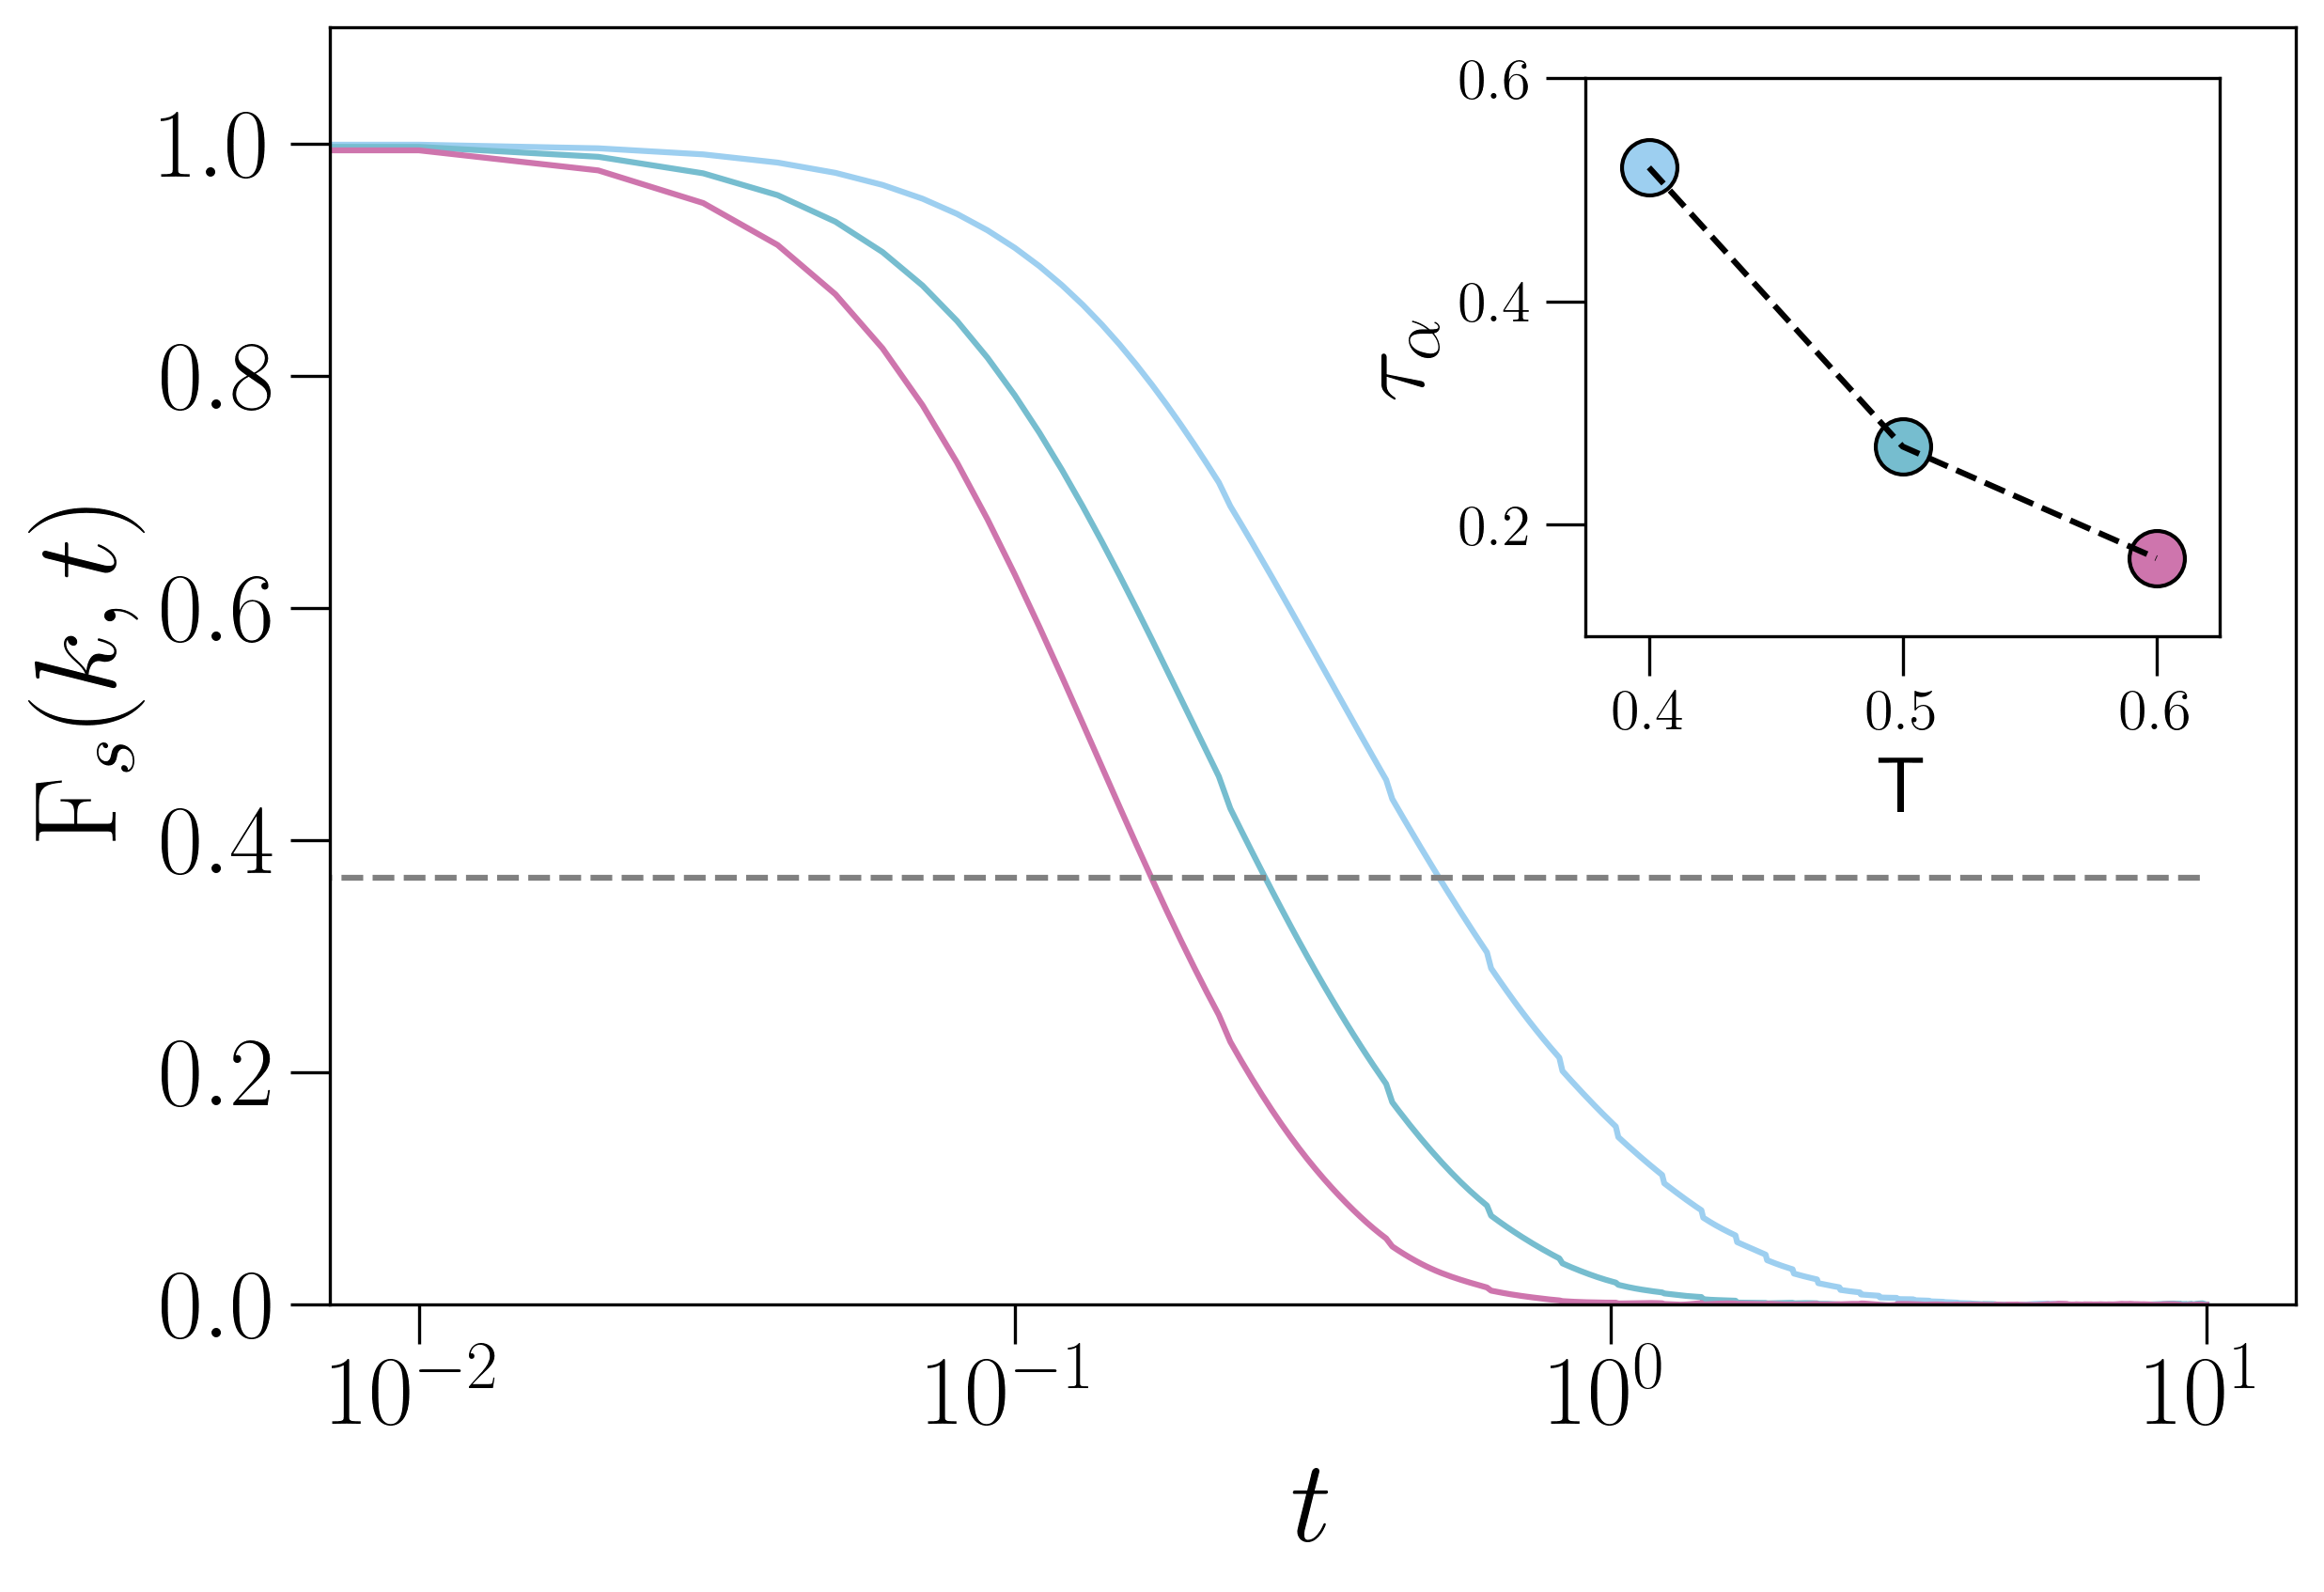
\includegraphics[width=0.8\linewidth]{chapters/colloids/figsColloids/figISF_example.png}
	\centering
	\caption[Intermediate scattering function.]{The self-part of the intermediate scattering function for an equilibrium fluid of soft repulsive spheres. Plotted for three temperatures: the function $F(k,t)$ relaxes from 1 to 0 as the system evolves. From these curves the structural relaxation time $\tau_\alpha$ can be determined when $F_s(k = 2\pi, \tau_{\alpha}) = e^{-1}$, shown in inset. Dotted line for $F_s(k,t) = e^{-1}$. }
	\label{fig:ISFs}

\end{figure*}

\textit{Intermediate scattering function ---} this two point dynamical measure quantifies the relaxation of density fluctuations in a particulate system. This is a density-density time averaged correlation function that gives the probability that a particle $j$ will be located at a certain position and at a certain time, given the origin of particle $i$ at time $t=0$. It takes the following form:

\begin{equation}
  	F(k, t)=\frac{1}{N}\left\langle\sum_{i,j}^{N} \exp \left[\mathrm{i} \mathbf{k} \cdot\left(\mathbf{r}_{j}(t)-\mathbf{r}_{i}(0)\right)\right]\right\rangle
\end{equation}

\noindent where $k$ is the wavevector $k=|\mathbf{k}|$, usually taken as $2\pi$. Often, only self-correlations are considered, in which case one can consider only the \textit{self} part of the intermediate scattering function:

\begin{equation}
  	F_{\mathrm{s}}(k, t)=\frac{1}{N}\left\langle\sum_{j}^{N} \exp \left[\mathrm{i} \mathbf{k} \cdot\left(\mathbf{r}_{j}(t)-\mathbf{r}_{j}(0)\right)\right]\right\rangle
\end{equation}


\noindent The relaxation of the system described through the decay of $F_s(k,t)$ defines a useful timescale; the structural relaxation time $\tau_{\alpha}$. This timescale provides a metric through which to understand the variation in the decay of density correlations across different state points and environments \cite{hansen2006}.
$\tau_{\alpha}$ can be defined as $F_s(k = 2\pi, \tau_{\alpha}) = e^{-1}$. An example of this function measured on an equilibrium fluid is plotted in Fig. \ref{fig:ISFs}. Here we can see that $F_s(k,t)$ relaxes on shorter timescales at higher temperatures, this is also seen in the reduction of the extracted structural relaxation time $\tau_\alpha$.



\textit{Overlap function ---} this dynamical measurement describes the evolution of the degree of \textit{overlap} between particle configurations. An overlap is defined as $w\left(\left|\mathbf{r}_{j}(0)-\mathbf{r}_{i}(t)\right|\right)$, where $i$, and $j$ are particle indices. This overlap is unity inside a region  $\left|\mathbf{r}_{j}(0)-\mathbf{r}_{i}(t)\right| \leq l$ and $0$ otherwise, where the distance $l$ is usually defined as $0.3 \sigma$. The overlap function measures this overlap $w$ for all particles between a configuration at time $t$ and the initial configuration at $t=0$: 


\begin{equation}	
	Q(t)=\frac{1}{N} \sum_{j=1}^{N} \sum_{i=1}^{N} w\left(\left|\mathbf{r}_{j}(0)-\mathbf{r}_{i}(t)\right|\right).
	\label{eq:Overlap}
\end{equation}

\noindent where $N$ is the number of particles. Therefore, $Q(t)$ measures degree of spacial similarity between a configuration with itself at a later time. The evolution of $Q$ describes relaxation in pinned systems, and can give indications of both dynamic and static correlations \cite{szamel2013}. 




\textit{Dynamic susceptibility ---} the variance of the overlap function $Q(t)$ defines the dynamic susceptibility $\chi_4$:

\begin{equation}
	\chi_{4}(t)=\frac{V}{N^{2} k_{B} T}\left[\left\langle Q^{2}(t)\right\rangle-\langle Q(t)\rangle^{2}\right],
	\label{eq:chi4}
\end{equation}

\noindent where $V$ is the system volume, $k_B$ is the Boltzmann constant and $T$ is the system temperature. $\chi_4$ is often used as a measure of dynamic heterogeneity, a feature of highly dense liquids in which some regions can move faster than others. When measured across a system, the peak of the $\chi_4$ distribution contains information as to the extent of dynamic heterogeneity within the system
%, defining both a dynamical correlation lengthscale as well as an indication as 
referring to the number of particles located in dynamically heterogeneous regions \cite{lacevic2003a}, and from which dynamical lengthscales can be inferred \cite{flenner2010}.


\subsection{Slow dynamics in random pinning liquids}
\label{section:SlowDynamics}

\begin{figure*}
	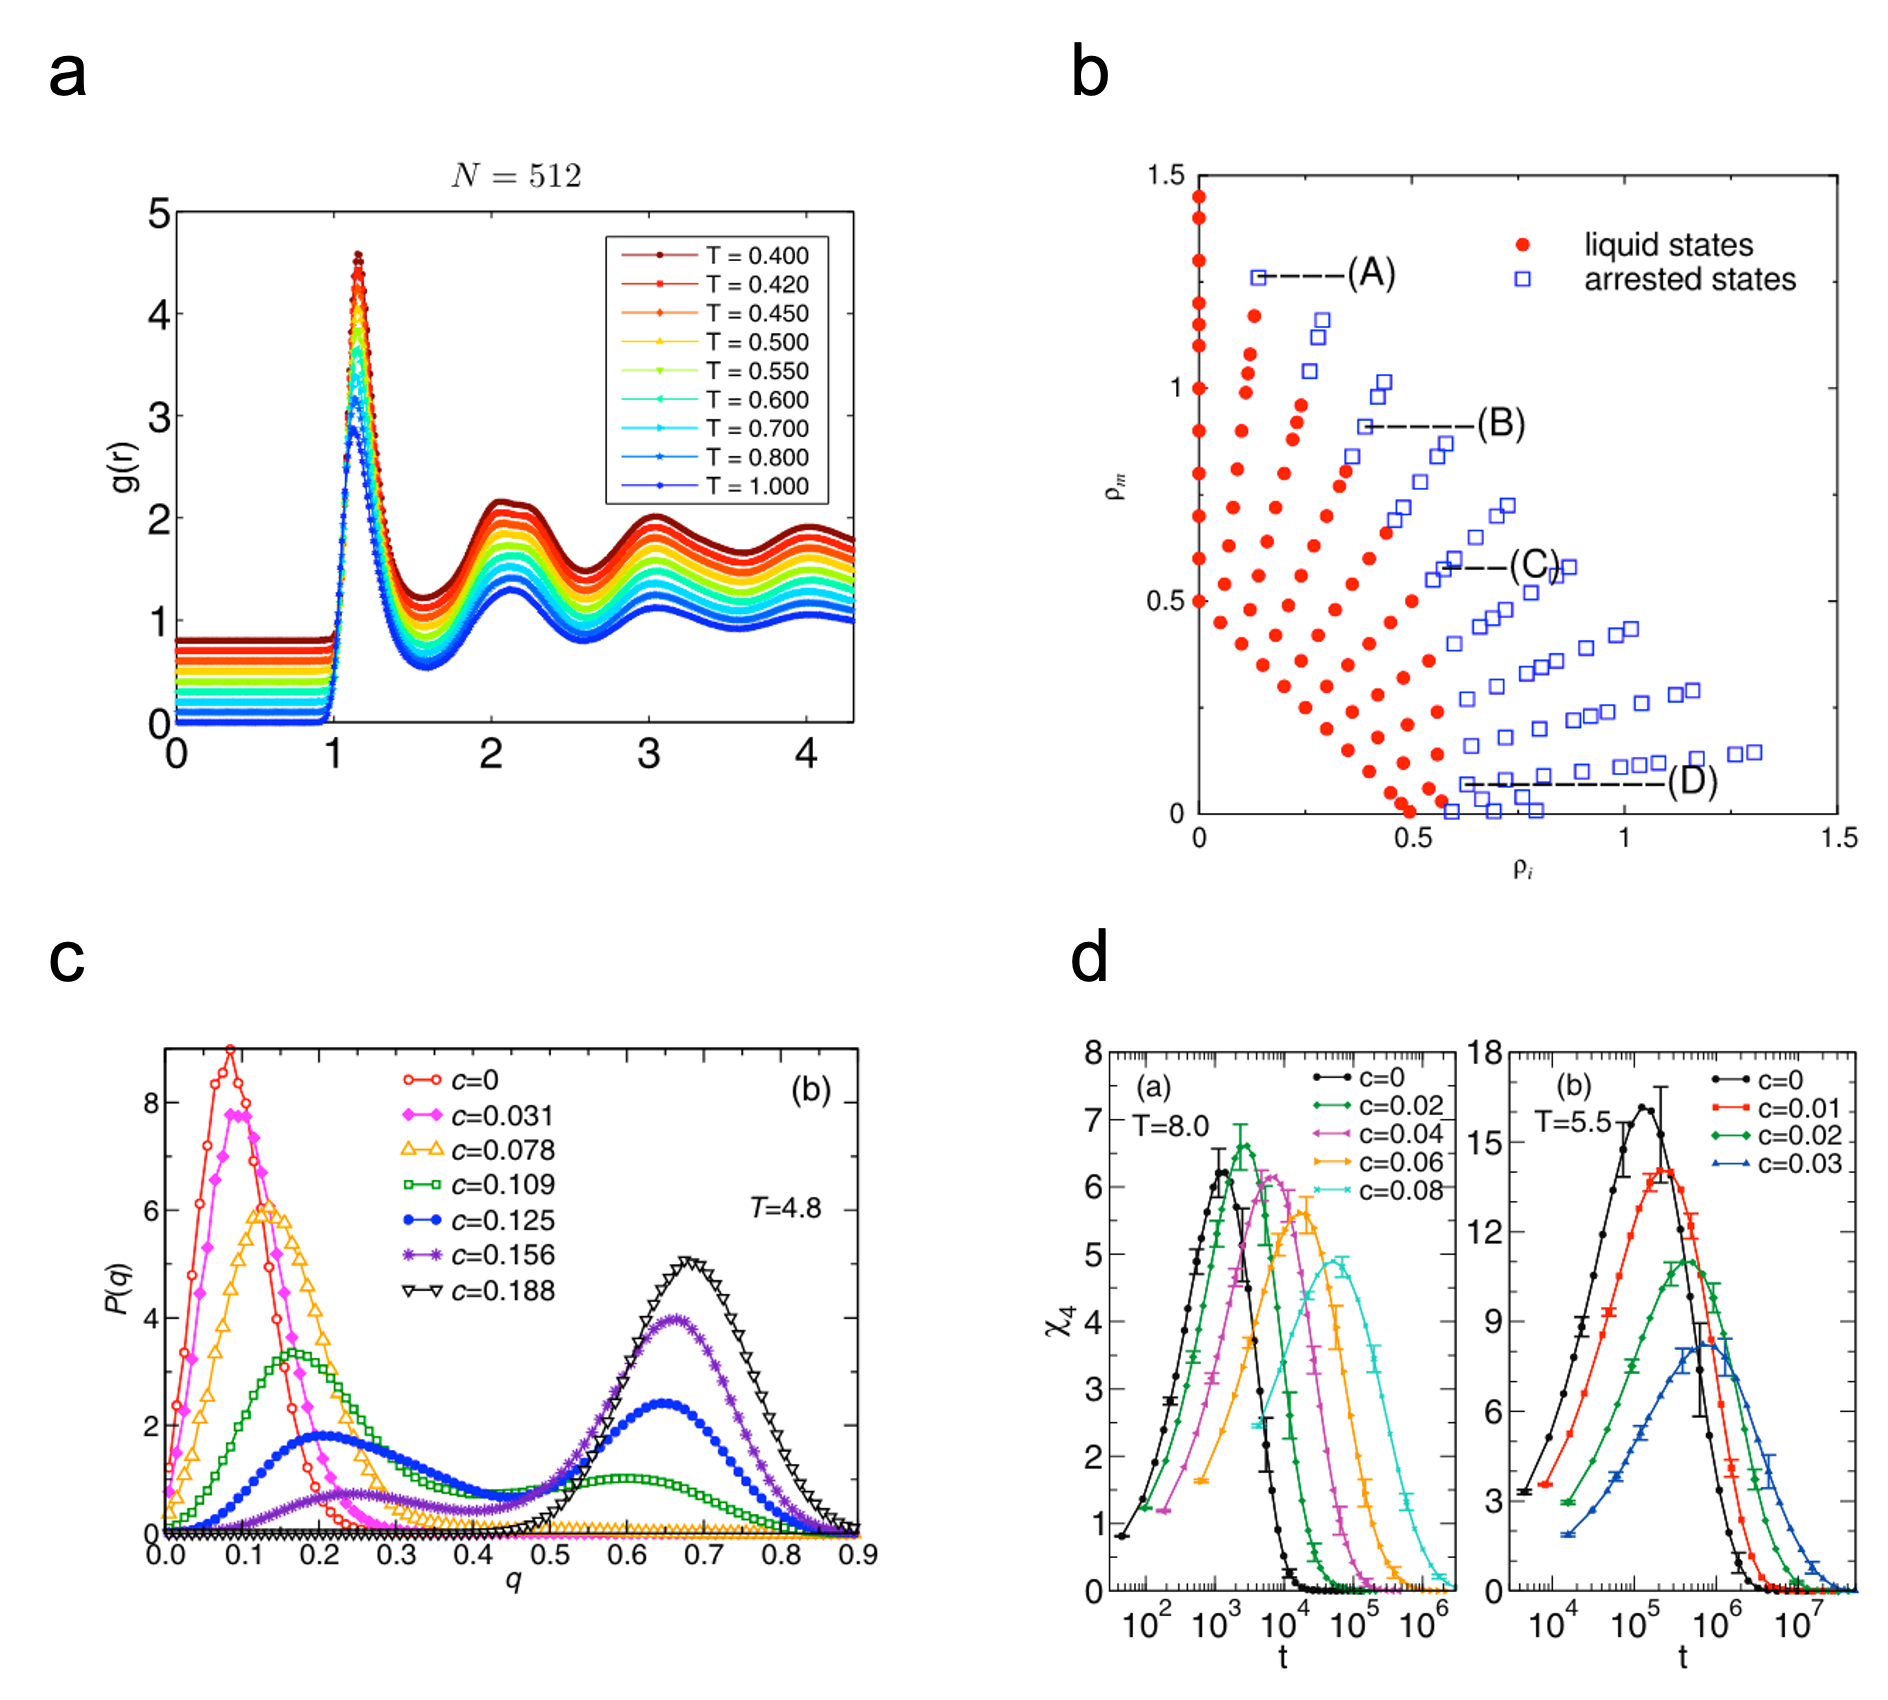
\includegraphics[width=\linewidth]{chapters/colloids/figsColloids/figPinning.png}
	\caption[Structural and dynamical response to  random pinning.]{Structural and dynamical response to  random pinning. \textbf{a} $g(r)$ analysis shows that pinning inhibits crystallisation in liquids at various temperatures, reproduced from ref. \cite{karmakar2013}. \textbf{b} Dynamic phase diagram for pinned liquids: where $\rho_i$ is the density of pinned particles, $\rho_m$ is the density of mobile particles. Arrested states correspond to ensembles where $\tau_{\alpha} > 10^3$, reproduced from ref. \cite{kim2011}. \textbf{c} Probability distribution of the overlap for various pinning fractions (c) shows two peaks at low temperatures, reproduced from ref. \cite{kob2013}. \textbf{d} Time dependence of $\chi_4$ for various pinning fractions (c) and two temperatures, shows the pinning cause a reduction in $\chi_4$. reproduced from ref. \cite{kob2014}.}
	\label{fig:Pinning}
\end{figure*}

In the previous chapter we introduced glasses: solid states of condensed matter with microscopic disorder. The formation of these materials happens through a glass transition, a process that occurs over inaccessible timescales. Therefore, to study the glass transition many have looked for methods to preserve the disordered phase at high density and accelerate the glass transition. For this random pinning can be used: if a random fraction of particles are pinned within a liquid at high temperature, and then that system is quenched (the system is rapidly cooled), then the frustration introduced into the system through pinning can be sufficient to maintain the disorder. This method may be seen as an expansion of the work originally conducted by Biroli \etal \cite{biroli2008}, that has now found wide-spread use \cite{cammarota2012,gokhale2014a,kob2014,li2015}. In Fig. \ref{fig:Pinning}a we show this method being employed by Karmarkar \etal \cite{karmakar2013}, where the preservation of disorder can be shown via the radial-distribution function $g(r)$.  

Interest in this system extends beyond glass physics, as it provides a convenient system through which to study fluids in random confined media and transport phenomena within random crowded environments. Kim \etal \cite{kim2011} studied the slow dynamics of supercooled liquids with various fractions of pinned particles. They report a dynamic phase diagram (Fig. \ref{fig:Pinning}b) wherein the system undergoes dynamical arrest as a function of increasing the fraction of pinned particles. 
In a similar system, the development of bimodality in the probability distribution of the overlap function was observed as a function of increasing the pinning fraction (Fig. \ref{fig:Pinning}c). This can be interpreted as a first-order transition to a phase coexistence between a low-overlap liquid and a high-overlap glass \cite{kob2013}. 
This behaviour is indicative of dynamic heterogeneity, Kob \etal \cite{kob2014} measure $\chi_4$ on randomly pinned liquids at various pinning fractions (Fig. \ref{fig:Pinning}d). Here we see the peak of these distributions moves to longer times as a function of increased pinning fraction, demonstrating the slowing of dynamics due to the presence of the pins. In addition, the peak of $\chi_4$ reduces with pinning fraction, here the pins reduce the effective size of relaxing regions and hence the dynamic heterogeneity in the system.

These works collectively demonstrate the primary characteristics of random pinning systems namely: the disruption of structural order; the slowing of dynamics up to dynamical arrest; the introduction of a random first-order phase transition; and the reduction of dynamic heterogeneity.  

